\documentclass{article}
\usepackage[hidelinks]{hyperref}
\usepackage{graphicx}
\usepackage{amsfonts}
\usepackage{amsmath}
\usepackage{enumitem}
\usepackage{polski}
\usepackage[utf8]{inputenc}
\usepackage{indentfirst}
\usepackage{float}
\title{Dokumentacja projektu dotyczącego optymalnego układania klocków na planszy}
\author{Abdelkarim Ahmed, Cacko Agata, Hernik Aleksandra}
\begin{document}
\maketitle
\section{Opis projektu}
\section{Opis algorytmu}
Wykorzystany algorytm jest algorytmem zachłannym z określoną parametrem liczbą nawrotów $k$. W każdym kroku algorytmu uruchamiane jest $k'$, gdzie $1 \le k' \le k$ (w sekcji wielowątkowość znajduje się wyjaśnienie, od czego jest uzależniona ich dokładna liczba). Każdemu wątkowi odpowiada jeden z $k$ najlepszych wyników uzyskanych w poprzednim kroku, gdzie najlepszy wynik to taki, dla którego wartość funkcji kosztu jest jak najmniejsza -- każdy z nich dla swoich danych wejściowych znajduje $k$ najlepszych rozwiązań. Znalezienie rozwiązań polega na sprawdzeniu dla każdego klocka każdego jego rotacji -- najpierw wybierana jest jego pozycja, a następnie liczony koszt całej planszy. $k$ rozwiązań takich, że funkcja kosztu obliczona na planszy z położonym danym klockiem w danej rotacji jest najmniejsza, to rozwiązanie dla danego wątku. Następnie, spośród ułożeń otrzymanych przez wszystkie wątki ($1 \le k' \le k$, zatem otrzymywane jest od $k$ do $k^2$ ułożeń) wybierane jest $k$ najlepszych. Ogólny schemat działania algorytmu podsumowuje poniższy diagram:
\begin{figure}[H]
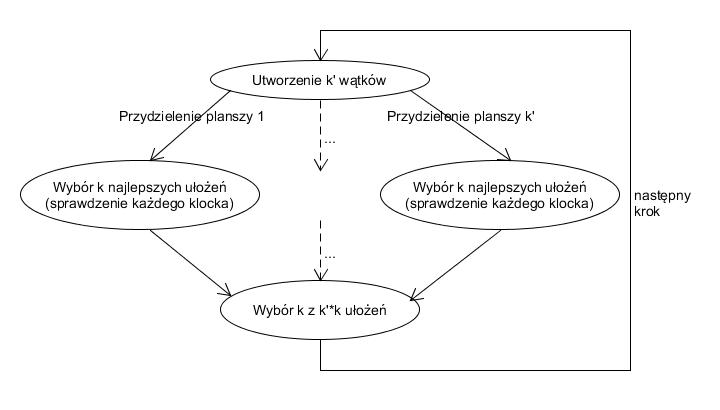
\includegraphics[width=\textwidth]{schemat_algorytmu.png}
\caption{Ogólny schemat działania algorytmu}
\end{figure}
\subsection{Wybór pozycji dla klocka}
\subsection{Funkcje kosztu planszy}
\subsection{Wielowątkowość}
W celu przyspieszenia działania algorytmu, do wykonywania niezależnych od siebie obliczeń wykorzystywany jest mechanizm wątków. W tym przypadku takimi obliczeniami jest szukanie $k$ najlepszych rozwiązań dla danej planszy. W każdym kroku tworzone jest $k'$ wątków, gdzie $1 \le k' \le k$, a w większości przypadków $k'=k$. 

Pierwszym ze szczególnych przypadków jest pierwszy krok - ponieważ jest tylko jedno wcześniejsze ułożenie (pusta plansza), uruchamiany jest tylko jeden wątek -- gdyby było uruchomione k wątków, każdy z nich znalazł by te same rozwiązania i w efekcie algorytm wybrałby najlepsze rozwiązanie z każdego wątku -- czyli wynikiem pierwszego kroku byłoby k identycznych ułożeń. Dzięki uruchomieniu tylko jednego wątku, znajdowane jest k różnych ułożeń, a ponadto, szczególnie dla dużych k, wykonuje się on szybciej. 

Drugi przypadek jest efektem dodatkowego usprawnienia algorytmu, który ma na celu eliminowanie identycznych rozwiązań, w celu sprawdzenia jak największej liczby możliwości. Polega ono na tym, że po każdym kroku sprawdzana jest unikalność rozwiązań -- sprawdzany jest najpierw ostatni położony klocek (współrzędne, w których został położony, obrót i identyfikator). Jeśli wykryty zostanie jakikolwiek konflikt, dokonywane jest porównanie plansz wynikowych. W przypadku, gdy plansze również są identyczne, pozostawiane jest tylko jedno z tych rozwiązań -- bo identyczne plansze dają identyczne rozwiązania, więc dopóki jakieś rozwiązanie pochodzące z tej planszy byłoby jednym z $k$ najlepszych istniejących, dwa wątki wykonywałyby dokładnie te same operacje. W ten sposób do następnego kroku może trafić zredukowana liczba plansz wejściowych, ale krok później, o ile znowu nie występowały powtórzenia, algorytm stabilizuje liczbę wątków na $k$. Koszt takiego rozwiązania jest niewielki -- porównanie wstępne jest realizowane w czasie stałym (liczba porównań jest rzędu $k^2$, gdzie $k$ to stała, a porównanie ułożenia klocka to cztery porównania liczb całkowitych), więc jeśli problem nie wystąpi, algorytm nie działa zauważalnie wolniej. Liczba sytuacji, w których trzeba wykonać dodatkowe sprawdzenie, powinna być bardzo niewielka, a eliminacja identycznych rozwiązań eliminuje jednakowe obliczenia, które mogłyby ciągnąć się nawet do samego końca -- efektywnie algorytm działałby od pewnego momentu tak, jakby wartość $k$ została zmniejszona.
\subsection{Łączenie wyników}
\subsection{Struktura danych}
\section{Testy}
%\subsection{zestaw pierwszy...}
%\subsection{zestaw drugi...}
\section{Wnioski} %z testów
\end{document}